\documentclass{article}
\usepackage{ctex}
\usepackage{graphicx}
\usepackage{amsmath}
\usepackage{indentfirst}
\usepackage{titlesec}
\usepackage{setspace}
\usepackage{subfigure}
\usepackage{caption}
\usepackage{float}
\usepackage{booktabs}
\usepackage{geometry}
\usepackage{multirow}
\geometry{left=1.2cm,right=1.2cm,top=2cm,bottom=2cm}
\title{\songti \zihao{2}\bfseries HW2第3题产生半球面均匀分布点实验报告}
\titleformat*{\section}{\songti\zihao{4}\bfseries}
\titleformat*{\subsection}{\songti\zihao{5}\bfseries}
\renewcommand\thesection{\arabic{section}}
\author{王启骅 PB20020580}
\begin{document}
	\maketitle
	\section{题目}
	在球坐标系 $ (\rho,\theta,\phi) $   下,产生上半球面上均匀分布的随机坐标点,给出
	其直接抽样方法。
	\section{算法原理}
由于在球面上产生,故取$ \rho=1 $,u,v为两个[-1,1]分布的均匀随机数列,则$ r=\sqrt{u^2+v^2} $,判断如果r<1则取该随机坐标。


根据
\begin{equation}
	x=2u\sqrt{1-r^2}
\end{equation}
\begin{equation}
	y=2v\sqrt{1-r^2}
\end{equation}
\begin{equation}
	z=1-2r^2
\end{equation}


转化为球坐标系
\begin{equation}
	\begin{cases}
		x=\sin\theta\cos\phi&\\
		y=\sin\theta\sin\phi&\\
		z=\cos\theta&
	\end{cases}
\end{equation}
并改为上半球面(z>0)为
\begin{equation}
	\theta=\arcsin(2r\sqrt{1-r^2})
\end{equation}
\begin{equation}
	\phi=
	\begin{cases}
		\arccos(u/r)& \text{,$v>0 $}\\
		\arcsin(v/r)+2\pi&\text{,$ u>0\ \&\ v<0 $}\\
		-\arccos(u/r)+2\pi&\text{,$ u<0\ \&\ v<0 $}
	\end{cases}
\end{equation}

	\section{结果}
一共产生$ 10^4 $个随机数点,并导入halfsphere.txt文件用python画出散点图
\begin{figure}[!h]
	
	\centering
	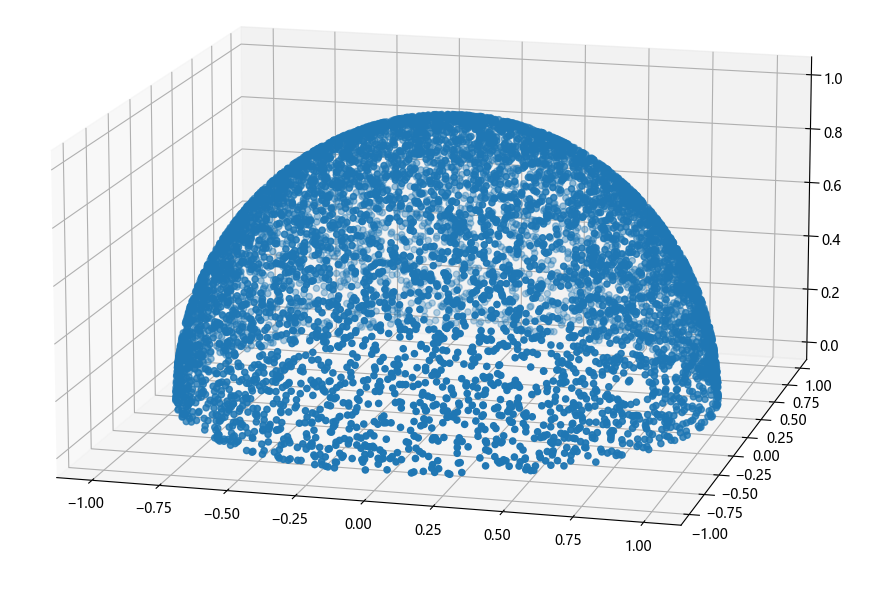
\includegraphics[scale=0.5]{result_3}
	\captionsetup{font={small},labelfont=bf}
	\caption{\heiti\zihao{-5}半球面均匀随机分布}
	
\end{figure}


	\section{结论}
	通过随机分布散点图可以看出该抽样法满足产生半球面上均匀分布的散点
\end{document}